\chapter{Test af accelerometer} 
\label{sec:test_acc}
I dette projekt anvendes to accelerometre, som er beskrevet i \autoref{sec:acc_teori}. Disse anvendes som sensorer til opsamling af acceleration, der giver et outputsignal i form af en spænding. For at kunne anvende et accelerometer er det vigtigt at kende forskellige tolerancer i forhold til deres datablade, hvorfor et forsøg udføres for at kunne tage højde for disse parametre.

\section{Formål}\label{sec:acc_formaal}
Denne test har til formål at identificere en given spænding for forskellige vinkler. Derudover identificeres %støjsignaler i outputsignalet samt 
offsettet og sensitiviteten for at teste accelerometrenes tolerancer.

\begin{enumerate}
%\item Identificering af støj i outputsignaler for accelerometrene
\item Test af linearitet
\item Identificering af offsettet for acceleromtrene %og sensitiviteten for accelerometrene
%\item Identificering af spænding ved forskellige vinkler
\end{enumerate}

\section{Materialer}
\begin{itemize}
\item Accelerometre ADXL$335$
\item Tape
\item Vaterpas
\item Breadboard
\item Vinkeltester, fremgår af \autoref{fig:vinkeltest}
\item Computer med Scopelogger og MATLAB
\item Spændingsforsyning på $3,4~V$ 
\item NI USB-6009
\end{itemize}

\section{Metode}
Der opstilles en metode til hvert formål i \autoref{sec:acc_formaal}. Formål 1 opfyldes ved deltest 1, og formål 2 opfyldes ved deltest 2.
\begin{enumerate}
%\item Der foretages målinger i accelerometerets tre akser og i de seks positioner som accelerometeret, hvorved støj som accelerometeret påvirkes med kan identificeres
\item Der foretages målinger i accelerometrets tre akser i 11 positioner, hvorved der testes for linearitet
\item Der foretages målinger i accelerometrets tre akser i de seks positioner, der ses af \autoref{sec:acc_fremgangsmaade}, hvorefter offset kan bestemmes ud fra målingerne. Offsettet bestemmes ud fra accelerometrets 0 g-påvirkning, der måles vinkelret på planet, hvilket svarer til at accelerometret ikke udsættes for tyngdekraften
% Sensitiviteten måles ud fra en 1 g-påvirkning
%\item Ud fra målingerne ved 0 og 1 g-påvirkning kan spændingen ved $1^{\circ}$ og $90^{\circ}$ beregnes ved \autoref{equ:vinkler}
\end{enumerate}

\section{Forsøgsopstilling}
Hver forsøgsopstilling udføres for begge accelerometre.

\subsection{Deltest 1}
\begin{itemize}
\item Accelerometret påsættes vinkeltesteren på \autoref{fig:vinkeltest}
\begin{itemize}
\item Accelerometret indstilles efter fremgangsmåden for hver øvelse, som er illustreret i \autoref{sec:vinkel_fremgangsmaade}
\end{itemize}
\item Accelerometret tilkobles NI USB-6009, der yderligere tilkobles en computer
\end{itemize}

\begin{figure}[H]
\centering
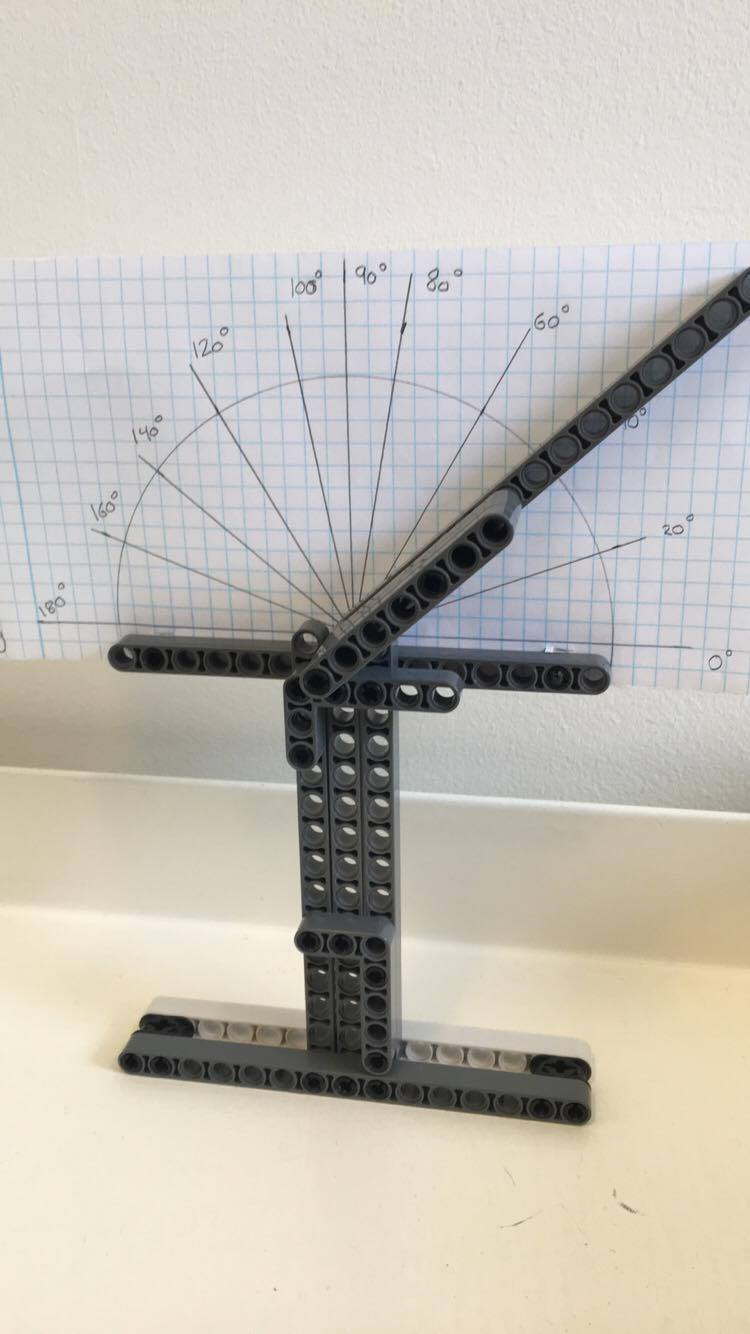
\includegraphics[width=0.6\textwidth]{figures/vinkeltest}
\caption{Vinkeltester, som anvendes under forsøget til at holde accelerometret i bestemte vinkler.}
\label{fig:vinkeltest}
\end{figure}

\subsection{Deltest 2}
\begin{itemize}
\item Accelerometret påsættes breadboardet med tape
\item Accelerometret stilles skiftevis vertikalt og horisontalt, således de forskellige akser testes
\begin{itemize}
\item Accelerometret placeres efter fremgangsmåden for hver øvelse, hvilket er illustreret af \autoref{sec:acc_fremgangsmaade}
\end{itemize}
\item Accelerometret tilkobles NI USB-6009, der yderligere tilkobles en computer
\end{itemize}

\section{Fremgangsmåde}  

\subsection{Deltest 1} \label{sec:vinkel_fremgangsmaade}
Vinkler på henholdsvis 0, 20, 40, 60, 80, 90, 100, 120, 140, 160 og $180^{\circ}$ måles og samples for hvert accelerometer i de tre akser i 10 sekunder ved $100~Hz$, hvilket er udregnet ud fra Nyquists sætning. Samplingsfrekvensen er dermed det dobbelte af båndbredden for accelerometrene \citep{analogdevices2010}. Målingerne er udført for begge accelerometre i henholdsvis X-, Y- og Z-aksen, og vinklen ændres ved at justere vinkeltesteren på \autoref{fig:vinkeltest}, så følgende vinkler fremgår af modellen:

\begin{itemize}
\item $0^{\circ}$ til $180^{\circ}$ med $20^{\circ}$'s intervaller
\item $90^{\circ}$  
\end{itemize}

\subsection{Deltest 2}\label{sec:acc_fremgangsmaade}
Der foretages målinger i seks forskellige positioner. Hver position måles tre gange og samles i 10 sekunder ved $100~Hz$. De forskellige positioner er illustreret i \autoref{sec:acc_imp} af \autoref{fig:acc}, og er som følger: 
\begin{itemize}
\item Accelerometret stilles lodret opad
\item Accelerometret stilles lodret nedad
\item Accelerometret stilles vandret mod højre
\item Accelerometret stilles vandret mod venstre
\item Accelerometret ligges plan på bordet med toppen opad
\item Accelerometret ligges plan på bordet med toppen nedad
\end{itemize}

\section{Resultater} 

\subsection{Deltest 1} \label{sec:resul_linear}
For deltest 1 udføres lineær regression, hvor data fra målingerne af begge accelerometres output ved hver målt vinkel plottes som en funktion af vinklerne. Derefter udføres den lineære regression, og $R^2$-værdien findes, så det kan bestemmes, om punkterne er lineære. Plots, regressioner og $R^2$-værdier kan ses på \autoref{fig:acc_lineaerregression}.

\begin{figure}[H]
\centering
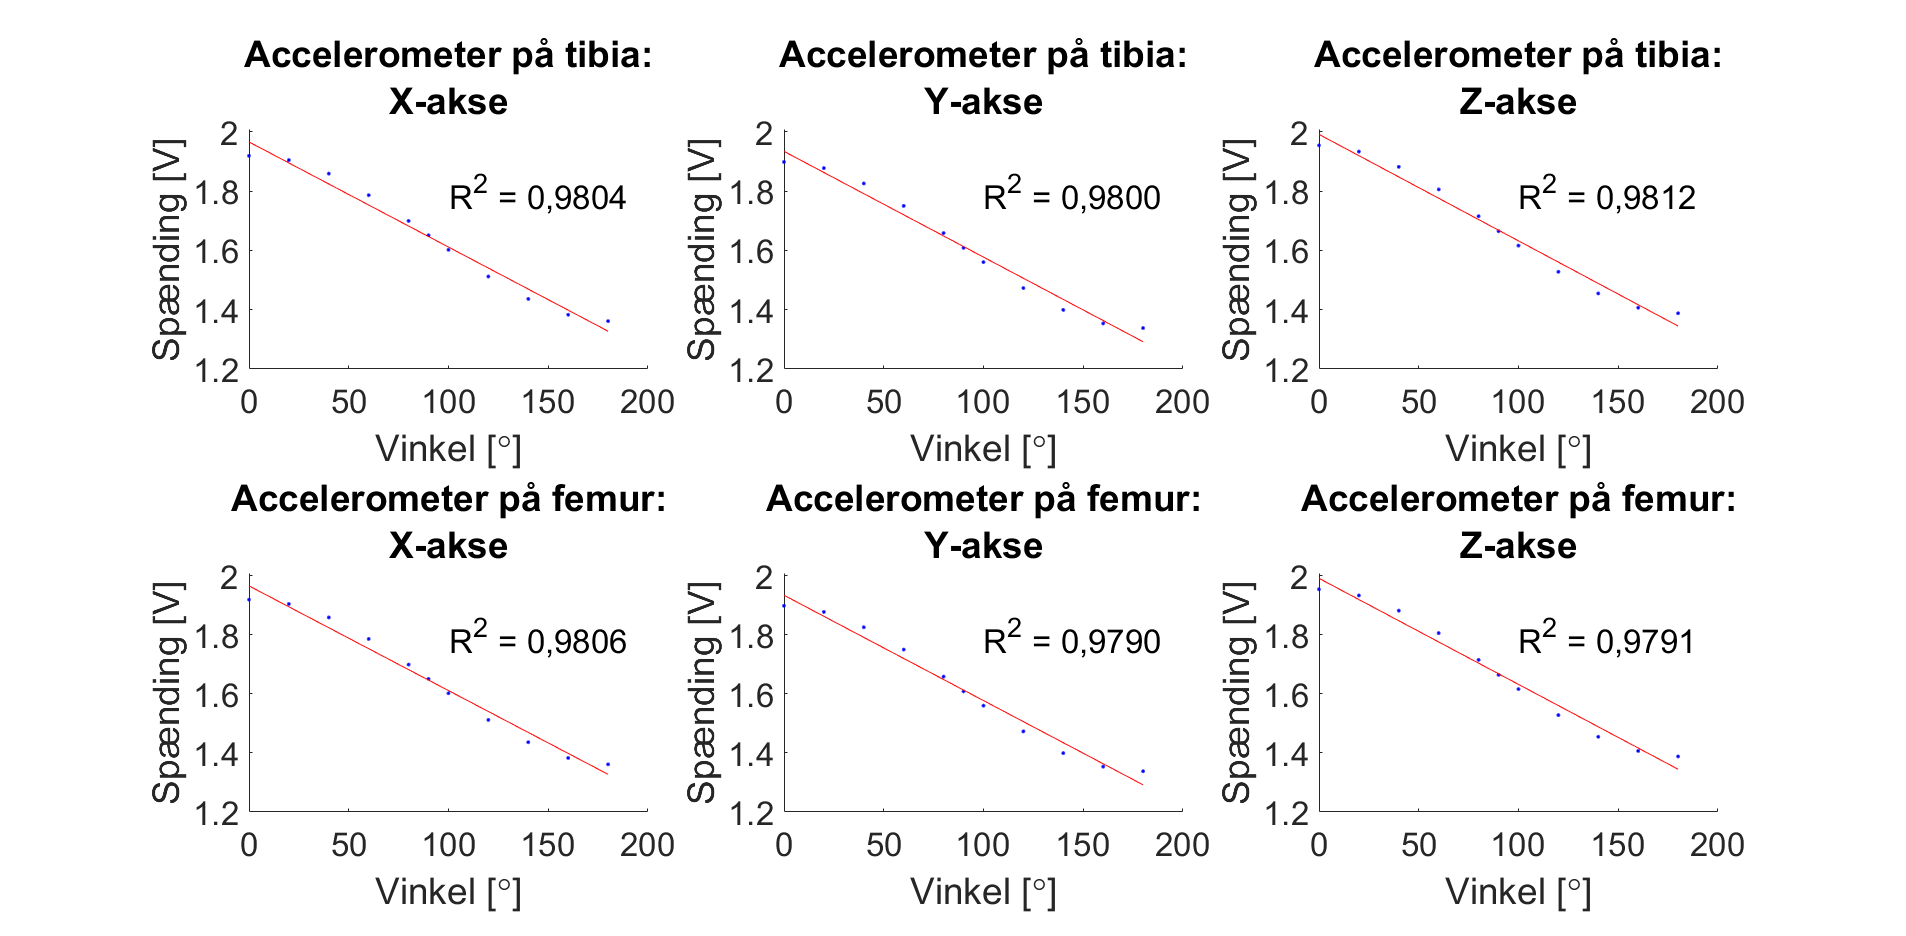
\includegraphics[width=1.0\textwidth]{figures/lineaerregression}
\caption{Lineær regression for hver akse på hvert accelerometer. Målingerne er plottet med blå prikker, og den lineære regression er illustreret med rød. $R^2$-værdien er angivet for hvert plot.}
\label{fig:acc_lineaerregression}
\end{figure}

\noindent
Ud fra \autoref{fig:acc_lineaerregression} kan det ses, at $R^2$-værdierne er mellem 0,9790 og 0,9812, hvilket svarer til, at sammenhængen er $2\%$ fra at være perfekt lineær. Graferne ville have en perfekt lineær sammenhæng, hvis $R^2=1$. Det kan derfor siges, at der her ses en lineær tendens ud fra disse målinger, selvom punkterne på alle seks grafer viser en s-formet bølge omkring regressionslinjen, hvilket giver afvigelserne fra den perfekte lineære sammenhæng.

\subsection{Deltest 2}
Ud fra de tre målinger foretaget i de seks forskellige positioner beregnes den gennemsnitlige værdi af målingerne på de forskellige akser, herefter plottes disse i. På denne måde bliver det muligt at se, hvilken akse der påvirkes mest under øvelsen. Målingerne fremgår af \autoref{fig:acc_paavirkning2}. 

\begin{figure}[H]
\centering
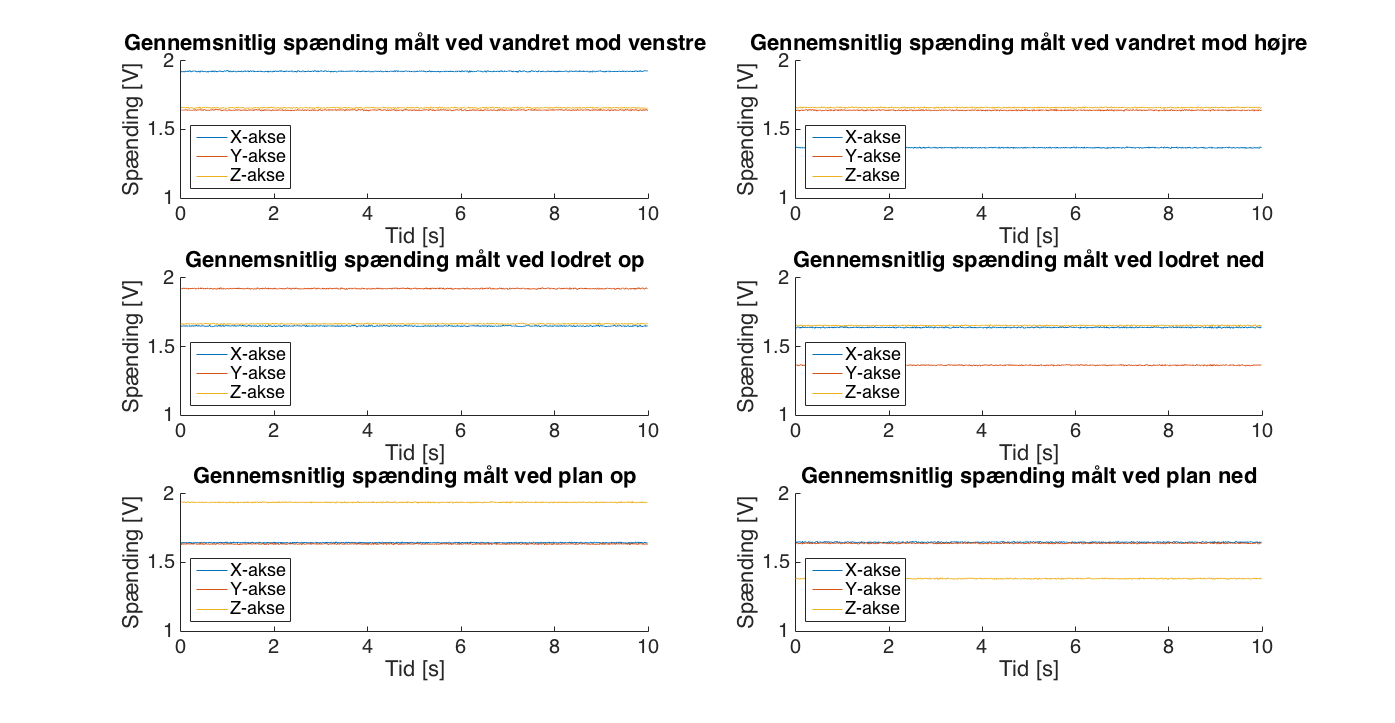
\includegraphics[width=1.0\textwidth]{figures/paavirkning}
\caption{Påvirkningen af accelerometrets tre akser ved de seks forskellige positioner.}
\label{fig:acc_paavirkning2}
\end{figure}

\noindent
Offset bestemmes ud fra de målinger, hvor accelerometret påvirkes i $0~g$-påvirkning. Den akse, hvor accelerometret påvirkes med 0 g i alle seks forskellige positioner fremgår af \autoref{fig:acc}. Resultaterne fra målingerne på Y-aksen ses på \autoref{tab:acc_offset}. 

\begin{table}[H]
	\centering
	\begin{tabular}{|l|l|l|} \hline
\textbf{Målt retning} & \textbf{Målt offset} & \textbf{Målt afvigelse} \\ \hline
    %\textbf{Lodret op} 		& X 		& $1,6793~V$ 	\\ \hline
   % \textbf{Lodret op} 		& Z 		& $1,6857~V$ 	 \\ \hline
    %\textbf{Lodret ned}		& X 		& $1,6750~V$ 	\\ \hline
    %\textbf{Lodret ned}		& Z 		& $1,6806~V$  	\\ \hline
    %\textbf{Vandret højre} 	& Y 		& $1,6760~V$    \\ \hline     
    %\textbf{Vandret højre} 	& Z 		& $1,6828~V$ 	\\ \hline
    %\textbf{Vandret venstre}	& Y 		& $1,6755~V$ 	\\ \hline
    %\textbf{Vandret venstre}	& Z 		& $1,6836~V$	\\ \hline
    %\textbf{Plan op} 			& X 		& $1,6773~V$	\\ \hline		
    \textbf{Positiv} 			& $1,6362~V$	& $3,75 \%$    \\ \hline
    %\textbf{Plan ned} 			& X 		& $1,6787~V$	\\ \hline
    \textbf{Negativ} 			& $1,6413~V$	& $3,45 \%$	\\ \hline
	\end{tabular}
	\caption{Offsettet for accelerometret, samt dens afvigelse i forhold til databladet bestemt for Y-aksen. Accelerometret udsættes for en 0 g-påvirkning i Y-planet.}
	\label{tab:acc_offset}
\end{table}

%Sensitiviten beregnes ud fra forskellen mellem 0 og 1 g-påvirkningen af accelerometeret. Der hvor accelerometeret er påvirket med 1 g er illustreret på \autoref{fig:acc_paavirkning}. Målingerne fremgår af \autoref{tab:acc_sensitivitet}. 
%
%\begin{table}[H]
%	\centering
%	\begin{tabular}{|l|l|l|}
%	\textbf{Målt retning} & \textbf{Målt akse} & \textbf{Sensitivitet} \\ \hline
%    \textbf{Lodret op} 		& Y		& $0,1092~V/g$ 	\\ \hline
%    \textbf{Lodret ned}		& Y 		& $-0,1164~V/g$ 	\\ \hline
%    %\textbf{Vandret højre} 	& X 		& $0,1130~V/g$     \\ \hline     
%    %\textbf{Vandret venstre}	& X 		& $-0,1167~V/g$ 	\\ \hline
%    %\textbf{Plan op} 		& Z 		& $0,1232~V/gV$    	\\ \hline		
%    %\textbf{Plan ned} 		& Z 		& $-0,1079~V/g$		\\ \hline
%	\end{tabular}
%	\caption{Sensitiviteten beregnet for Y-aksen, hvor accelerometeret udsættes for en 1 g-påvirkning.}
%	\label{tab:acc_sensitivitet}
%\end{table}
%
%Ud fra senstitivten beregnes spændingen ved $1^{\circ}$ og $90^{\circ}$ i negativ og positiv retning\fxnote{Er der nødvendig med 1 grad?}. Spændingen svarende til $0^{\circ}$ svarer til den målte offsetværdi som fremgår af \autoref{tab:acc_offset}. Udregningerne af spænding ved de valgte grader fremgår af \autoref{tab:acc_grader} og er beregnet ud fra ligning \autoref{equ:vinkler}.
%
% \begin{table}[H]
%	\centering
%	\begin{tabular}{|l|l|l|l|}
%	\textbf{Målt retning} & \textbf{Målt akse} & \textbf{Spændingen ved $0^{\circ}$} & \textbf{Spændingen ved $90^{\circ}$} \\ \hline
%    \textbf{Positiv} 	& Y		& $1,7985~V$   	&	$12,7589~V$\\ \hline
%    \textbf{Negativ}	& Y		& $1,5692~V$  	&	$-8,0339~V$\\ \hline
%   % \textbf{Positiv} 	& X 		& $1,7917~V$   	& 	$11,5105~V$ \\ \hline     
%    %\textbf{Negativ}	& X 		& $1,5614~V$		&	$-8,7982~V$\\ \hline
%    %\textbf{Positiv} 	& Z 		& $1,7924~V$   	& 	$11,8494~V$	\\ \hline		
%    %\textbf{Negativ} 	& Z 		& $1,5629~V$		&	$-8,8190~V$ \\ \hline
%	\end{tabular}
%	\caption{Beregnet spænding ved henholdsvis $0^{\circ}$ og $90^{\circ}$ i positiv og negativ retning.}
%	\label{tab:acc_grader}
%\end{table}





